% Created 2017-07-26 Wed 14:47
\documentclass[a4paper]{article}
\usepackage[utf8]{inputenc}
\usepackage[T1]{fontenc}
\usepackage{fixltx2e}
\usepackage{graphicx}
\usepackage{longtable}
\usepackage{float}
\usepackage{wrapfig}
\usepackage{rotating}
\usepackage[normalem]{ulem}
\usepackage{amsmath}
\usepackage{textcomp}
\usepackage{marvosym}
\usepackage{wasysym}
\usepackage{amssymb}
\usepackage{hyperref}
\tolerance=1000
\usepackage{minted}
\usepackage[margin=0.8in]{geometry}
\usepackage{amssymb,amsmath}
\usepackage{fancyhdr} %For headers and footers
\pagestyle{fancy} %For headers and footers
\usepackage{lastpage} %For getting page x of y
\usepackage{float} %Allows the figures to be positioned and formatted nicely
\floatstyle{boxed} %using this
\restylefloat{figure} %and this command
\usepackage{hyperref}
\hypersetup{urlcolor=blue}
\usepackage{minted}
\setminted{frame=single,framesep=10pt}
\chead{}
\rhead{\today}
\cfoot{}
\rfoot{\thepage\ of \pageref{LastPage}}
\author{Nathan Hughes (\href{mailto:nah31@aber.ac.uk}{nah31@aber.ac.uk})}
\date{\today}
\title{QTL Mapping Notes}
\hypersetup{
  pdfkeywords={},
  pdfsubject={},
  pdfcreator={Emacs 24.5.1 (Org mode 8.2.10)}}
\begin{document}

\maketitle
\maketitle
\clearpage
\tableofcontents
\clearpage





\section{What is QTL Analysis?}
\label{sec-1}
Quantitative Trait Locus  Analysis is a statistical method that links two types of information
\begin{itemize}
\item Phenotypic data (i.e. trait measurements)
\item Genotypic data (usually molecular markers)
\end{itemize}

\subsection{What is a single QTL}
\label{sec-1-1}
An individual QT is a secton of DNA, it is arbitrarily described by correlation and not a physical element that can be seen. 

\subsection{What is it used for?}
\label{sec-1-2}
QTL attempts to explain the genetic basis of variation in complex traits. 
They allow researches in many fields, from agriculture to evolutionary biology, to link complex phenotypes to specific 
regions of chromosomes. 

\subsection{What is the goal of it?}
\label{sec-1-3}
The end goal of the QTL process is to identify the action, interaction number, and precise location of regions on a chromosome 
which "code" for specific phenotypic expression
\\
\\
More specifically the principle goal is to answer the question of whether phenotypic differences are primarily due to few loci with farily
large effects, or to many loci, each with minute effects. It appears that a substantial proportion of the phenotypic variation in many quantitative 
traits can be explained with few loci of large effect, with the remainder due to numerous loci of small effect. 
For example, in domesticated rice (Oryza sativa), studies of flowering time have identified six QTL; the sum of the effects
of the top five QTL explains 84\% of the variation in this trait. 

\section{What can you do with QTL Data}
\label{sec-2}
Once QTL have been identified, molecular techniques can be employed to narrow the QTL down to candidate genes. One important
emerging trend in these analyses is the prominent role of regulatory genes, or genes which code for transcription factors and other 
signalling proteins. For instance, in rice, three flowering time QTL have been identified at the molecular level, and all of these loci 
encode regulatory proteins know from studies of \emph{Arabidopsis thaliana}.

\begin{center}
\begin{figure}[htb]
\centering
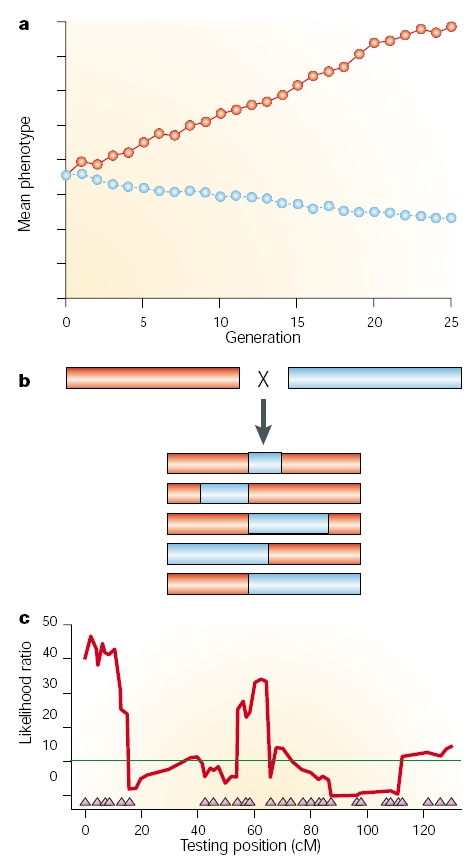
\includegraphics[width=0.3\textwidth,height=0.5\textwidth]{./images/qtl.jpg}
\caption{\label{fig:QTL-Data}© 2001 Nature Publishing Group Mackey, T. F. Quantitative trait loci in Drosophila. Nature Reviews Genetics 2, 13 (2001). All rights reserved}
\end{figure}
\end{center}

\section{How does QTL work?}
\label{sec-3}
In order for QTL to be conducted, two things are required: 
\begin{enumerate}
\item Two or more strains of organisms which differ genetically with regard to the trait of interest (Fig1. a shows variation in a population over time).
\begin{itemize}
\item For example selecting lines which have alleles that influence flowering colour.
\end{itemize}
\item Genetic markers for that specific species  which distinguish between parental lines.
\begin{itemize}
\item Molecular markers are preferred for genotyping, because these markers are unlikely to affect the trait of interest.
\end{itemize}
\end{enumerate}

\section{Generating populations for study}
\label{sec-4}
This involves using the identified parents/individuals/organisms and running a breeding program to build up a population suitable 
for use in genetic difference identification.

\subsection{Initial selection and crossing}
\label{sec-4-1}
Carrying out the QTL analysis is done by crossing the, genetically different, identified strains and a $f^1$ population of \textbf{heterozygous} 
individuals is produced (Fig 1. B). These are then selectively chosen and used to produce further generations to a $f^n$ generation.
Next the genotypes' and phenotypes' of the $f^n$ generation individuals are scored. Markers that are genetically linked to a QTL influencing
the trait of interest will segregate more frequently with the trait values (flowering colour, in the previously mentioned example). Whereas unlinked markers
will not show significant association with phenotype (Fig 1. C). 

\subsection{Multi-gene traits}
\label{sec-4-2}
For traits controlled by tens or hundreds of genes, the paternal lines need not actually be different for the phenotype in question; 
rather they must simply contain different alleles, which are then resorted by recombination in the derived population to produce 
a range of phenotypic values. Consider for example, a trait which is controlled by four genes, wherein the upper-case alleles increase the value 
of the trait being studied. The lower-case alleles decrease the vale of that trait. Here, if the effects of the alleles of the four genes are 
similar, individuals with the AABBccdd and aabbCCDD genotypes might have roughly the same phenotype measurement. The members of the $f^1$ population 
(AaBbCcDd) would be invariant and would have an intermediate phenotype. However the $f^2$ generation, or the progeny from a backcross would have
anywhere from zero to eight upper-case alleles. The backcross progeny would have anywhere from four to eight upper-case alleles. 

\subsection{Problems with population sizes}
\label{sec-4-3}
A small population size may lead to problems and as such is a critical factor to the validity of experiments. A small sample size may 
lead to overestimation of the effect of a QTL. 

\section{Types of markers}
\label{sec-5}
As mentioned there are several different kinds of markers, these are just a few commonly used examples
\subsection{SNPs}
\label{sec-5-1}
Single nucleotide polymorphisms, are the most common type of genetic variation among people. Each SNP represents a difference in a single 
DNA building block (nucleotide). For example a SNP may replace the nucleotide cytosine (C) with the nucleotide thymine (T) in a certain 
region of DNA. 

\begin{itemize}
\item The wikipedia article on this is quite good: 
\begin{itemize}
\item \url{https://www.wikiwand.com/en/SNP_genotyping}
\end{itemize}
\end{itemize}

\subsection{SSR}
\label{sec-5-2}
Simple sequence repeats, these have the ability to be done at a medium throughput. 

\subsection{RFLPs}
\label{sec-5-3}
Restriction fragment length polymorphisms. These were used as the primary markers up to the late 80's but couldn't be done 
through automated means, was expensive and thus became obsolete.


\section{Performing QTL Analysis with a set of markers}
\label{sec-6}
\section{\href{dictonary.org}{Biology Dictonary}}
\label{sec-7}
% Emacs 24.5.1 (Org mode 8.2.10)
\end{document}